\chapter{Zásuvný modul}
\label{4-plugin}

V~této kapitole je popsán samotný zásuvný modul. Pro~názornost a~srozumitelnost jsou zde uvedeny důležité části kódu a~diagramy znázorňující složitější algoritmy. Během~vývoje zásuvného modulu bylo čerpáno z~literatury zabývající se programem QGIS \citep{pyqgis_book}~\citep{qgis_book}, programovacím jazykem Python \citep{dive_into_python} \citep{python3_oop_book} a modulem PyQt \citep{pyqt_book}.

\section{Instalace}
\label{instalace}

Zásuvný modul není součástí oficiálního repozitáře QGIS, přesto ho lze nainstalovat stejným způsobem jako~jiné pluginy. Stačí do~programu QGIS přidat repozitář organizace GeoForAll Lab\footnote{http://geomatics.fsv.cvut.cz/research/geoforall/}. Nejprve je tedy nutné otevřít okno s~repozitáři \textit{Zásuvné moduly $\rightarrow$ Spravovat a~instalovat zásuvné moduly $\rightarrow$ Nastavení} (viz obr.~\ref{fig:pridani_repozitare}) a~zde pomocí tlačítka \textit{Přidat...} doplnit repozitář GeoForAll Lab dostupný na~adrese \url{http://geo.fsv.cvut.cz/geoforall/qgis-plugins.xml} (viz obr.~\ref{fig:pridani_repozitare_geoforall_lab}). Zásuvný modul se řadí mezi experimentální, proto je zapotřebí aktivovat volbu \textit{Zobrazit také experimentální zásuvné moduly}, viz obr.~\ref{fig:pridani_repozitare}. Poté už stačí do~vyhledávacího pole zadat \textit{PU Plugin} a~zásuvný modul pro pozemkové úpravy nainstalovat (viz obr. \ref{fig:instalace_puplugin}).

	\begin{figure}[H]
		\centering
		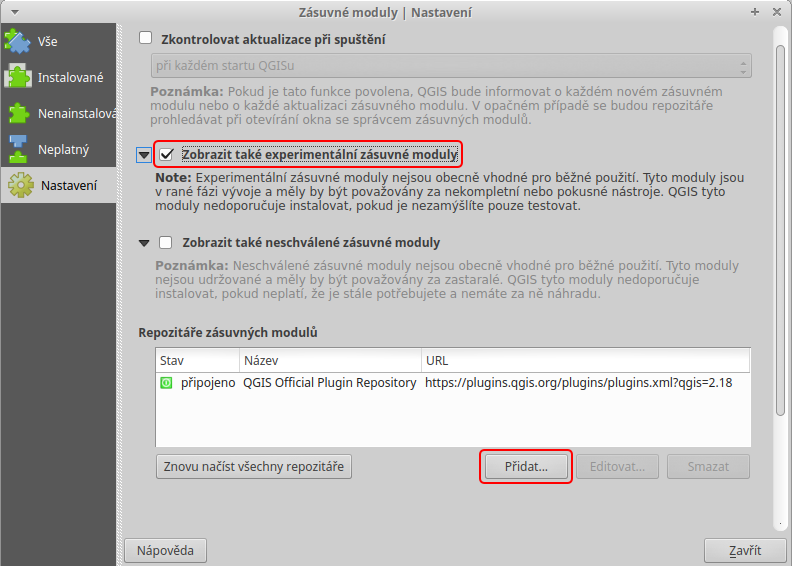
\includegraphics[width=.8\textwidth]{./pictures/pridani_repozitare.png}
		\caption[Přidání repozitáře]{Přidání repozitáře}
		\label{fig:pridani_repozitare}
 	\end{figure}
 	
	\begin{figure}[H]
		\centering
		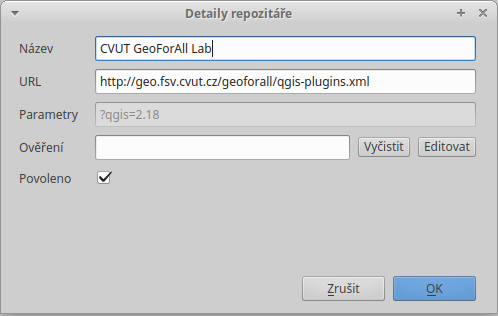
\includegraphics[width=.6\textwidth]{./pictures/pridani_repozitare-geoforall_lab.png}
		\caption[Přidání repozitáře GeoForAll Lab]{Přidání repozitáře}
		\label{fig:pridani_repozitare_geoforall_lab}
 	\end{figure}

	\begin{figure}[H]
		\centering
		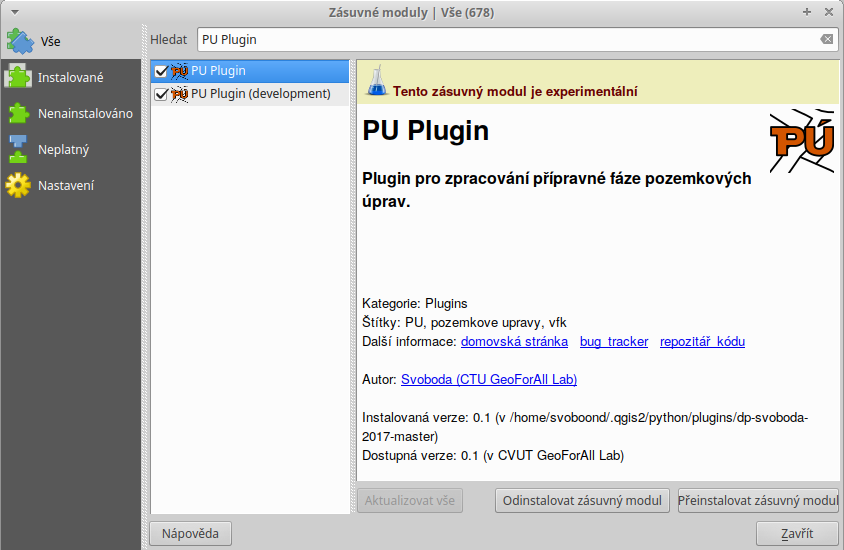
\includegraphics[width=.6\textwidth]{./pictures/instalace_puplugin.png}
		\caption[Instalace zásuvného modulu]{Instalace zásuvného modulu}
		\label{fig:instalace_puplugin}
 	\end{figure}

Když je plugin nainstalován, objeví se v~liště zásuvných modulů jeho ikona (viz obr.~\ref{fig:ikona_puplugin}). Okno zásuvného modulu je možné vyvolat poklepáním na~jeho ikonu nebo volbou \textit{Zásuvné moduly $\rightarrow$ PU Plugin $\rightarrow$ PU Plugin}.

	\begin{figure}[H]
		\centering
		
\includegraphics[width=.1\textwidth]{./pictures/puplugin.png}
		\caption[Ikona zásuvného modulu]{Ikona zásuvného modulu}
		\label{fig:ikona_puplugin}
 	\end{figure}

\section{Grafické uživatelské rozhraní}
\label{gui}

Grafické uživatelské rozhraní zásuvného modulu je reprezentováno jedním oknem (viz obr. \ref{fig:main_gui}), které je možné ukotvit do samotného programu QGIS.

	\begin{figure}[H]
		\centering
		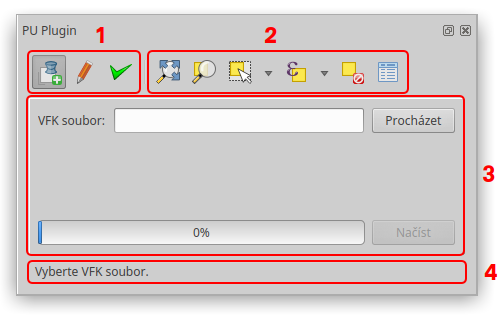
\includegraphics[width=.7\textwidth]{./pictures/main_gui.png}
		\caption[Grafické uživatelské rozhraní zásuvného modulu]{Grafické uživatelské rozhraní zásuvného modulu}
		\label{fig:main_gui}
 	\end{figure}

\begin{description}
	\item[Prvek 1:] Skupina tří ikon pro přepínání mezi záložkami:
	\begin{itemize}[leftmargin=1.5cm, noitemsep]
		\item \img{./pictures/loadvfk.png} \textit{Načtení VFK souboru}
		\item \img{./pictures/edit.png} \textit{Editace}
		\item \img{./pictures/checkanalysis.png} \textit{Kontroly a analýzy}
 	\end{itemize}
 	
	\item[Prvek 2:] Skupina nástrojů, které jsou propojené se standardními nástroji programu QGIS. Pokud tedy uživatel například aktivuje nástroj pro~výběr prvků polygonem v~okně zásuvného modulu, automaticky se aktivuje stejný nástroj v~panelu QGISu a~naopak.
	\begin{itemize}[leftmargin=1.5cm, noitemsep]
		\item \img{./pictures/zoom_full.png} \textit{Přiblížit na rozměry okna}
		\item \img{./pictures/zoom_to_selected.png} \textit{Přiblížit na výběr}
		\item tlačítko interaktivního výběru prvků z mapového okna
		\begin{itemize}[leftmargin=1.5cm, noitemsep]
			\item \img{./pictures/select_rectangle.png} \textit{Vybrat prvky oblastí nebo jednoklikem}
			\item \img{./pictures/select_polygon.png} \textit{Vybrat prvky polygonem}
			\item \img{./pictures/select_freehand.png} \textit{Vybrat prvky kreslením od ruky}
			\item \img{./pictures/select_radius.png} \textit{Vybrat prvky poloměrem}
 		\end{itemize}
		\item tlačítko výběru prvků
		\begin{itemize}[leftmargin=1.5cm, noitemsep]
			\item \img{./pictures/select_expression.png} \textit{Vybrat pomocí vzorce...}
			\item \img{./pictures/select_value.png} \textit{Vybrat prvky hodnotou...}
			\item \img{./pictures/select_all.png} \textit{Vybrat všechny prvky}
			\item \img{./pictures/invert_selection.png} \textit{Převrátit výběr prvků}
 		\end{itemize}
		\item \img{./pictures/deselect.png} \textit{Zrušit výběr prvků ve všech vrstvách}
		\item \img{./pictures/open_table.png} \textit{Otevřít atributovou tabulku}
 	\end{itemize}
	\item[Prvek 3:] Okna záložek zobrazující se v~závislosti na~tom, která ze~tří ikon prvku~1 je aktivní.
	\item[Prvek 4:] Stavový řádek, ve~kterém se ukazují zprávy pro~uživatele.
\end{description}

\section{Komunikace s uživatelem}
\label{komunikace}

Zásuvný modul komunikuje s uživatelem třemi způsoby:

\begin{enumerate}[leftmargin=1.5cm, noitemsep]
	\item \underline{Stavový řádek} (viz prvek~4 obr.~\ref{fig:main_gui}) představuje nejčastější způsob zobrazování zpráv zásuvného modulu. Pokud  uživatel neví jak postupovat, zde s~největší pravděpodobností najde potřebné informace. Běžné zprávy mají černou barvu písma, důležíté zprávy se~zobrazují červeně (viz obr.~\ref{fig:dulezita_zprava}).
	
	\begin{figure}[H]
		\centering
		
\includegraphics[width=.23\textwidth]{./pictures/statusbar-red_message.png}
		\caption[Důležitá zpráva ve stavovém řádku]{Důležitá zpráva ve stavovém řádku}
		\label{fig:dulezita_zprava}
 	\end{figure}	

	\item \underline{Pole zpráv} je standardní způsob komunikace mezi programem QGIS a uživatelem. Zobrazuje pole v horní části mapového okna, které může být nastaveno tak, že po určité době samo zmizí, nebo vyžaduje zavření uživatelem. Zprávy mají čtyři urovně zobrazení, viz tab. \ref{tab:urovne_pole_zprav}.

\begin{table}[H]
    \begin{tabular}{|l|l|}
        \hline
         úroveň & český popis \\
        \hline
        \hline
         INFO & informační zpráva \\ \hline
         WARNING & zpráva upozornění \\ \hline
         CRITICAL & kritická zpráva \\ \hline
         SUCCESS & zpráva úspěchu \\
         \hline
    \end{tabular}
    \centering
    \caption[Úrovně zobrazení pole zpráv]{Úrovně zobrazení pole zpráv (zdroj:~\citep{qgis_api})}
    \label{tab:urovne_pole_zprav}
\end{table}

Zásuvný modul využívá této komunikace pouze pro zobrazení významných zpráv, které by neměly být uživatelem opomenuty (viz obr. \ref{fig:zprava_pole_zprav}).

	\begin{figure}[H]
		\centering
		
\includegraphics[width=.8\textwidth]{./pictures/message_bar-message.png}
		\caption[Zpráva upozornění v poli zpráv]{Zpráva upozornění v poli zpráv}
		\label{fig:zprava_pole_zprav}
 	\end{figure}

	\item \underline{Logování} je posledním prostředkem pro~předávání informací, který zásuvný modul používá. Informace v~anglickém jazyce, zejména chybové hlášky, zapisuje do vlastní záložky s~názvem \textit{PU Plugin} (viz obr. \ref{fig:logovaci_panel}). Panel logovacích zpráv lze zobrazit kliknutím na~ikonu \img{./pictures/log.png} v~pravém dolním rohu QGISu.

	\begin{figure}[H]
		\centering
		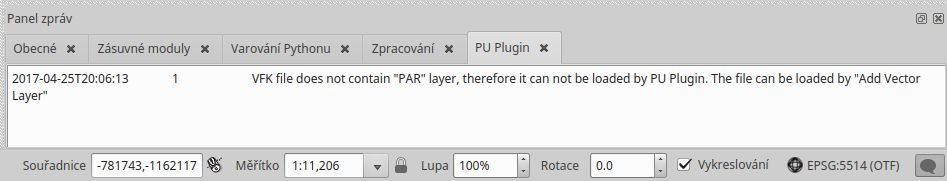
\includegraphics[width=1.0\textwidth]{./pictures/log_panel.png}
		\caption[Panel logovacích zpráv]{Panel logovacích zpráv}
		\label{fig:logovaci_panel}
 	\end{figure}

\end{enumerate}

\section{Načtení VFK souboru}
\label{nacteni_vfk}

%% digitalizace pomoci pluginu

%%BPEJ je zjednodusene - viz 9.8 http://www.spucr.cz/frontend/webroot/uploads/files/2015/12/metodickynavodkprovadenipozemkovychuprav1327.pdf